\documentclass[11pt, a4paper]{article}
\usepackage{graphicx}
\usepackage{amsmath}
\usepackage{listings}


\title{Assignment No 9:The Discrete Fourier Transform}

\author{G Ch V Sairam , EE19B081}

\date{05-05-2021}
\begin{document}		
		
\maketitle
\section*{Introduction}
This week’s assignment is based on Discrete Fourier Transform (DFT) of signals. We examine the DFT of various functions using the fft library in numpy. We also attempt to approximate the CTFT of a gaussian by changing the window size and number of samples until the error is below a threshold.

\section*{FFT and IFFT}
There are two commands in Python, one to compute the forward fourier transform and the other to compute the inverse transform.
They are np.fft.fft and np.fft.ifft respectively.
\newline
We find the Fourier transform and invert it back to the time domain for a random signal, find maximum error to test the reconstruction.
\begin{verbatim}
x=np.random.rand(100)
X=np.fft.fft(x)
y=np.fft.ifft(X)
print ("Absolute Maximum Error = ",abs(x-y).max())
\end{verbatim}
Doing this , we get the output:
\begin{verbatim}	
Absolute Maximum Error =  3.413079373551675e-16
\end{verbatim}

Printing out x and y side-by-side, we observe that the vectors are not exactly the same. x is purely real whereas y is slightly complex. This is due to the finite accuracy of the CPU so that the ifft could not exactly undo what fft did.

\section*{Spectrum of sin(5t)}
Here, we try to estimate the DFT of a sinusoidal function. For example,
\begin{equation*}
y=sin(x) = (exp(jx) - exp(-jx))/2j
\end{equation*}
The expected spectrum is,
\begin{equation*}
Y=(\delta(w-1) - \delta(w+1))/2j
\end{equation*}
In a similar process , we try to plot the spectrum of sin(5t).

\begin{figure}[!tbh]
\centering
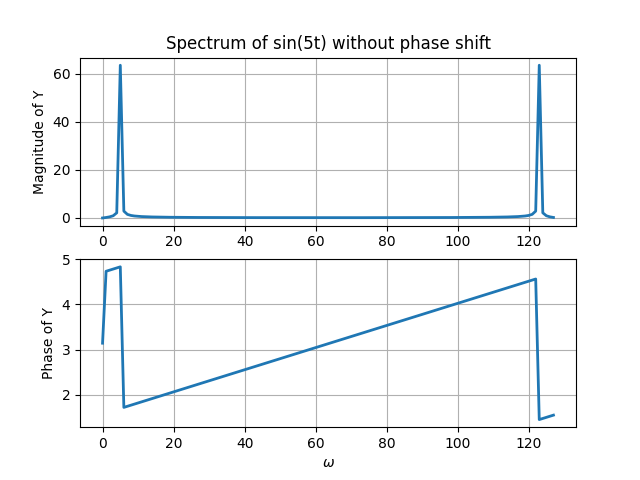
\includegraphics[scale=0.5]{assgn9_plot1.png} 
\label{fig1}
\end{figure} 

But, there are multiple issues to be fixed here:
\begin{itemize}
\item The peaks are not where we expect them to be. This can be corrected using fft shift.
\item The spikes have a height of 64, not 0.5. This should be rectified by dividing by the sample rate.
\item The frequency axis is not in place. This is due to the duplicacy of 0
and 2$\pi$.
\item The actual phase at the spikes is near but not exactly correct.
\end{itemize}

After doing these modifications , we get a much neater spectrum:
\begin{verbatim}
x=np.linspace(0,2*pi,129);x=x[:-1]
y=np.sin(5*x)
Y=np.fft.fftshift(np.fft.fft(y))/128.0
plt.figure()
plt.subplot(2,1,1)
plt.plot(w,abs(Y),lw=2)
plt.xlim([-10,10])
plt.subplot(2,1,2)
plt.plot(w,np.angle(Y),'ro',lw=2)
ii=np.where(abs(Y)>1e-3)
plt.plot(w[ii],np.angle(Y[ii]),'go',lw=2)
plt.xlim([-10,10])
\end{verbatim}

\begin{figure}[!tbh]
\centering
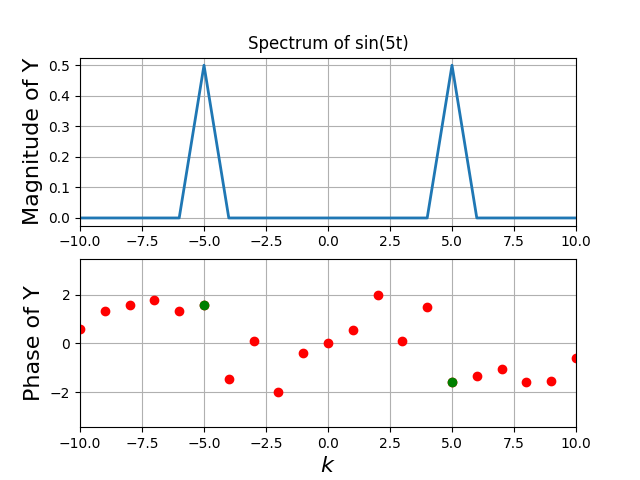
\includegraphics[scale=0.5]{assgn9_plot2.png} 
\label{fig2}
\end{figure} 

\section*{Spectrum of (1+0.1cos(t))cos(10t)}
We consider the amplitude modulated spectrum:
\newline
y=(1+0.1cos(t))cos(10t)
\newline
We expect a shifted set of spikes, with a main impulse and two side impulses on each side. This is because,
\begin{equation*}
0.1cos(10t)cos(t) = 0.05(cos11t + cos9t) = 0.025(exp(9jt)+exp(11jt)+exp(-9jt)+exp(-11jt))
\end{equation*}
\newline
Again, we use 128 points and generate the spectrum.

\begin{figure}[!tbh]
\centering
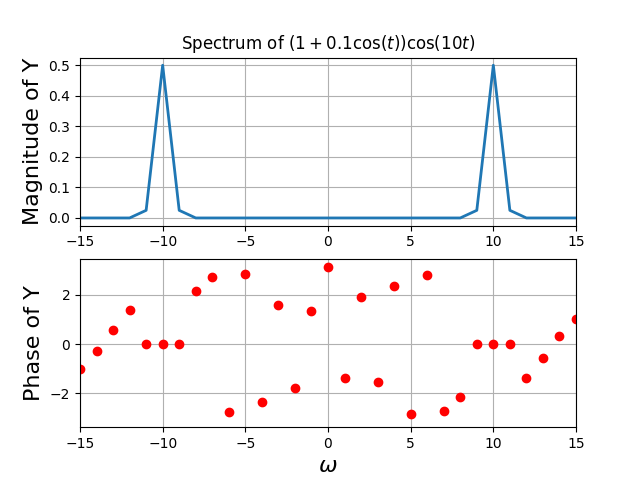
\includegraphics[scale=0.55]{assgn9_plot3.png} 
\label{fig3}
\end{figure} 

We see only a single broader spike. In order to see even the side peaks, the frequency resolution has to be improved. We can do so by keeping the number of samples constant and increasing the range in the time domain. The following spectrum is obtained:

\begin{figure}[!tbh]
\centering
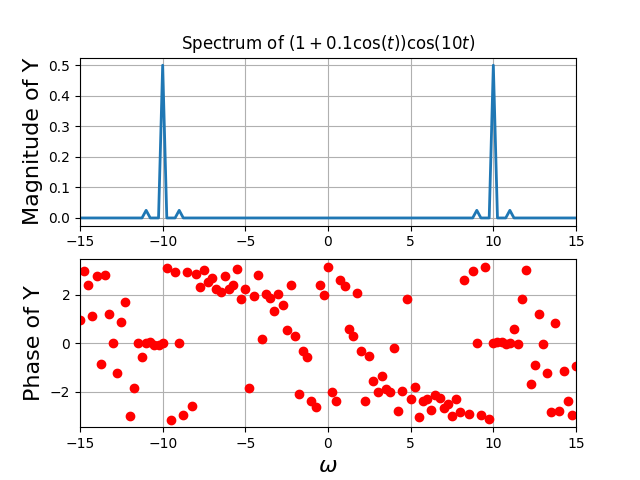
\includegraphics[scale=0.8]{assgn9_plot4.png} 
\label{fig4}
\end{figure} 
At all 3 peaks, the phase is 0 as expected for a cosine wave.

\section*{Assignment Questions}

\subsection*{Spectrum of $sin^3(t)$ and $cos^3(t)$}
Consider the sinusoids $sin^3(t)$ and $cos^3(t$) :
\begin{equation*}
sin^3(t)=(3sin(t)-sin(3t))/4
\end{equation*}
\begin{equation*}
cos^3(t)=(cos(3t)+3cos(t))/4
\end{equation*}
Thus, in the frequency spectrum, there will be 4 impulses at frequencies 1 and 3.
\newline
Taking the same precautionary measures as done previously, we obtain the following approximate spectrum :

\begin{figure}[!tbh]
\centering
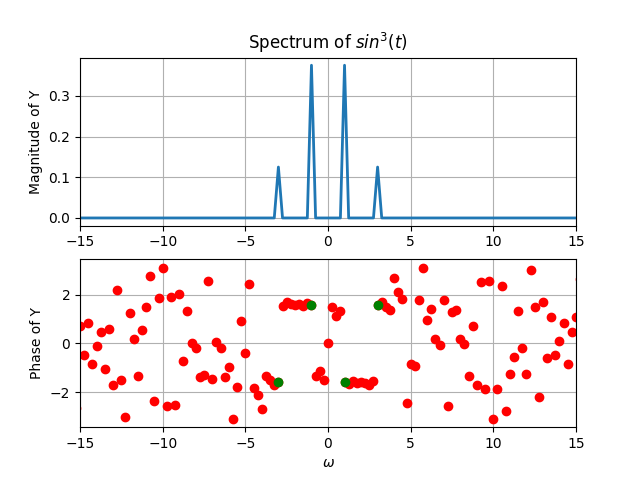
\includegraphics[scale=0.75]{assgn9_plot5.png} 
\label{fig5}
\end{figure} 

\begin{figure}[!tbh]
\centering
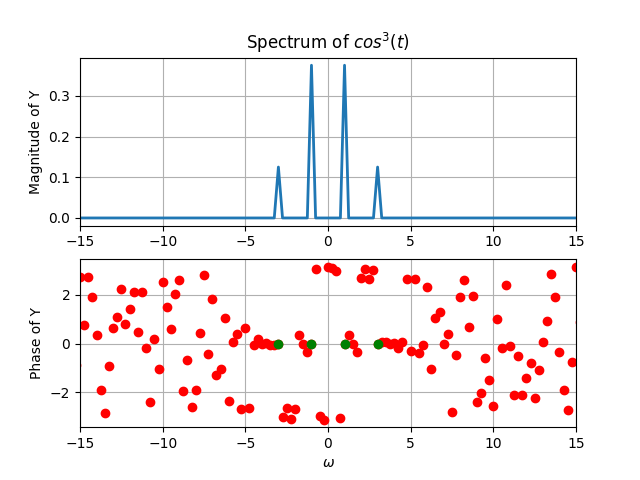
\includegraphics[scale=0.8]{assgn9_plot6.png} 
\label{fig6}
\end{figure} 
We observe that:
\newline
For $sin^3(t)$ , the phase is similar to that of sum of 2 sinusoids.
\newline
For $cos^3(t)$ , phase =0 at the peaks

\subsection*{Spectrum of frequency modulated wave}
Consider the signal:
\newline
f(t) = cos(20t + 5cos(t))
\newline
Because the argument of the cosine function itself consists of a cosine term, the wave can be expressed using Bessel functions. Thus, the frequency spectrum consists of impulses at the carrier frequency ($w_c$ = 20 here) and impulses at multiple side band frequencies, that are close to the carrier frequency.
\newline
Following the process same as above , we get:
\begin{figure}[!tbh]
\centering
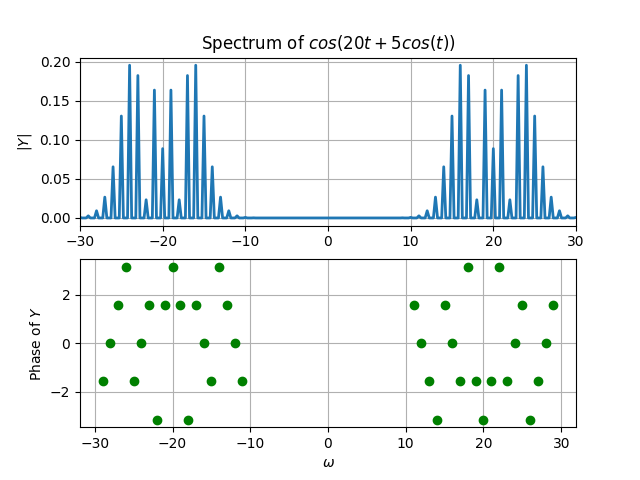
\includegraphics[scale=0.75]{assgn9_plot7.png} 
\label{fig7}
\end{figure} 

\subsection*{Spectrum of the Gaussian function}
The Gaussian function f(x) = $exp(-x^2/2)$ is not band-limited,in the sense that the frequency spectrum has non zero values even for very large frequencies. The Continuous Time Fourier Transform for the Gaussian is given by:
\begin{equation*}
F(jw)=\sqrt(2\pi) exp(-w^2 /2)
\end{equation*}
Thus, the phase is zero for all w while the magnitude is a Gaussian function.
\newline
We can make approximations by making the window size T larger, and by decreasing the time domain sampling period or increasing the number of samples N . We find the appropriate values for these iterative keeping the sampling frequency constant.

\begin{verbatim}
wlim=5
tolerance=1e-6
T = 8*pi
N = 128
Yold=0
err=1+tolerance
iters = 0
error=[]

#To find the optimum time range to get an accurate frequency domain.

while err>tolerance:  
	x = np.linspace(-T/2,T/2,N+1)[:-1]
	w = np.linspace(-N*pi/T,N*pi/T,N+1)[:-1]
	y = gauss(x)
	Y=np.fft.fftshift(np.fft.fft(np.fft.ifftshift(y)))*T/N
	Y_exp=expectedgauss(w)
	err = np.max(np.abs(Y[::2]-Yold))
	error.append(np.max(np.abs(Y-Y_exp)))
	Yold=Y
	iters+=1
	T*=2
	N*=2
	
error = np.max(error)
print("True Error: ",error)
print("Samples, N = "+str(N)+"\n"+"Time Period,T = "+str(int(T/pi))+"pi")

#Estimate DFT of gaussian function. Plot its magnitude and phase.

mag = np.abs(Y)
phi = np.angle(Y)

plt.figure()
plt.subplot(2,1,1)
plt.plot(w,mag,lw=2)
plt.xlim([-wlim,wlim])
plt.subplot(2,1,2)
ii=np.where(mag>1e-3)
plt.plot(w[ii],phi[ii],'go',lw=2)
plt.show()

#Expected DFT of Gaussian is a Gaussian in w. Hence, we plot the magnitude and phase of gaussian in w.

Y_exp = expectedgauss(w)   
mag_exp = np.abs(Y_exp)
phi_exp = np.angle(Y_exp)

plt.figure()
plt.subplot(2,1,1)
plt.plot(w,mag_exp,lw=2)
plt.xlim([-wlim,wlim])
plt.subplot(2,1,2)
ii=np.where(mag_exp>1e-3)
plt.plot(w[ii],phi_exp[ii],'go',lw=2)
plt.show()
\end{verbatim}

After the iteration, we find out the values of the number of samples and the Time Period as follows:
\begin{verbatim}
Samples, N = 512
Time Period,T = 32pi
\end{verbatim}

For these values , we get the error value in the order of 1e-15 .
\newline
Plotting the fft of estimated and expected gaussian functions , we get :

\begin{figure}[!tbh]
\centering
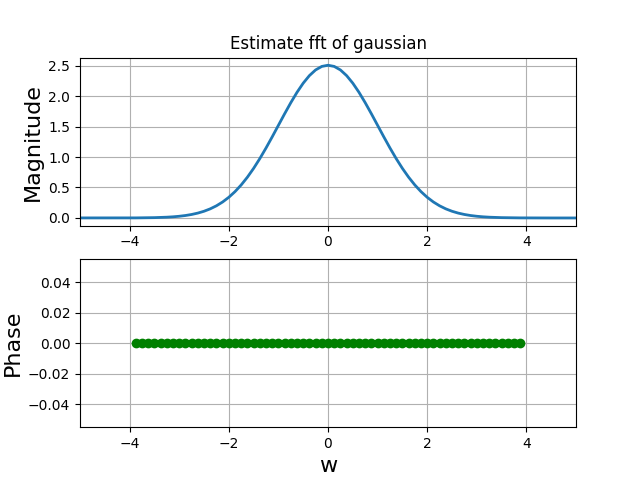
\includegraphics[scale=0.8]{assgn9_plot8.png} 
\label{fig8}
\end{figure} 

\begin{figure}[!tbh]
\centering
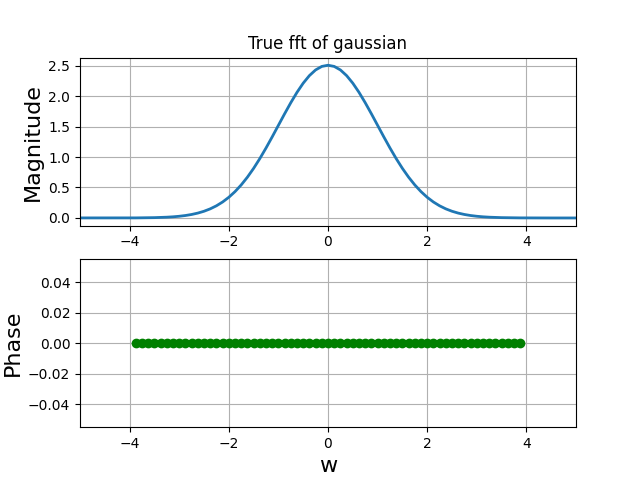
\includegraphics[scale=0.8]{assgn9_plot9.png} 
\label{fig9}
\end{figure} 

\section*{Conclusion}
The fft library in python provides a useful toolkit for analysis of DFT of signals. The Discrete Fourier Transforms of sinusoids, amplitude modulate signals, frequency modulated signals were analysed. In the case of pure sinusoids, the DFT contained impulses at the sinusoid frequencies. The amplitude modulated wave had a frequency spectrum with impulses at the carrier and the side band frequencies. The frequency moduated wave, having an infinite number of side band frequencies, gave rise a DFT with non zero values for a broader range of frequencies. The DFT of a gaussian is also a gaussian and the spectrum was found to sharpen for higher sampling rates, while broaden for greater time ranges. 

\end{document}